
\begin{frame}
  \frametitle{Testing Protocol}
  \begin{adjustwidth}{-15pt}{0pt}
  \vspace{-5pt}
  \begin{block}{Scikit-Learn Algorithms:}
    \begin{enumerate}
      \itemsep 0.2em 
      \footnotesize
      \item Scale training data ($0$ mean and unit variance)
      \item 5-fold cross val is used to iteratively remove 20\% of the train-set as a test-set
      \item \texttt{fit} and \texttt{predict} takes place, ground truth and predictions are tracked
      \item Each label is predicted separately
    \end{enumerate}
  \end{block}
  \pause
  \vspace{-5pt}
  \begin{block}{Maximum Log Likelihood:}
    \begin{enumerate}
      \itemsep 0.2em 
      \footnotesize
      \item Training database broken up into 10k segments (CHTC)
      \item Every training database entry is tested
      \item Testing sample removed from DB during each calculation
      \item Entire set of labels (reactor type, burnup, etc) predicted at once
    \end{enumerate}
  \end{block}
  \pause
  \vspace{-5pt}
  \begin{block}{SFCOMPO Testing with Nuclide Mass Training Set:}
    \begin{enumerate}
      \itemsep 0.2em 
      \footnotesize
      \item After filtering out for irrelevant cases, 505 test entries remain
      \item Training set units are converted to $mg/gU_i$
      \item In scikit, scaling is applied to the training set and testing set features
      \item MLL converts the units but doesn't require scaling
      \item Time since irradiation not included in SFCOMPO
    \end{enumerate}
  \end{block}
  \end{adjustwidth}
\end{frame}

\begin{frame}
  \frametitle{Reactor Type Classification Performance}
  \textbf{Accuracy Metrics:} \cite{scikit}
  \vspace{2mm}
  \begin{itemize}\addtolength{\itemsep}{0.4\baselineskip}
    \item $\uncover<1->{\textit{accuracy} = }
           \uncover<4->{\frac{1}{N_\text{samples}}}
           \uncover<3->{\sum_{i=1}^{N_\text{samples}}}
           \uncover<2->{\mathbb{I}(y_{pred,i} = y_{true,i})}$
    \item $\uncover<1->{\textit{balanced-accuracy} = }
           \uncover<5->{\frac{1}{\sum_{i}{w_i}}}
           \uncover<3->{\sum_{i=1}^{N_\text{samples}}}
           \uncover<5->{w_i \cdot}
           \uncover<2->{\mathbb{I}(y_{pred, i} = y_{true, i})}$ \\
          \hspace{1.1cm} \uncover<6->{where:} \uncover<6->{$w_i = \frac{1}{\sum_j{\mathbb{I}(y_j = y_i)w_j}}$}
    \uncover<7->{\item Confusion matrices:}
  \end{itemize}
  \invisible<-6>{\begin{figure}
    \centering
    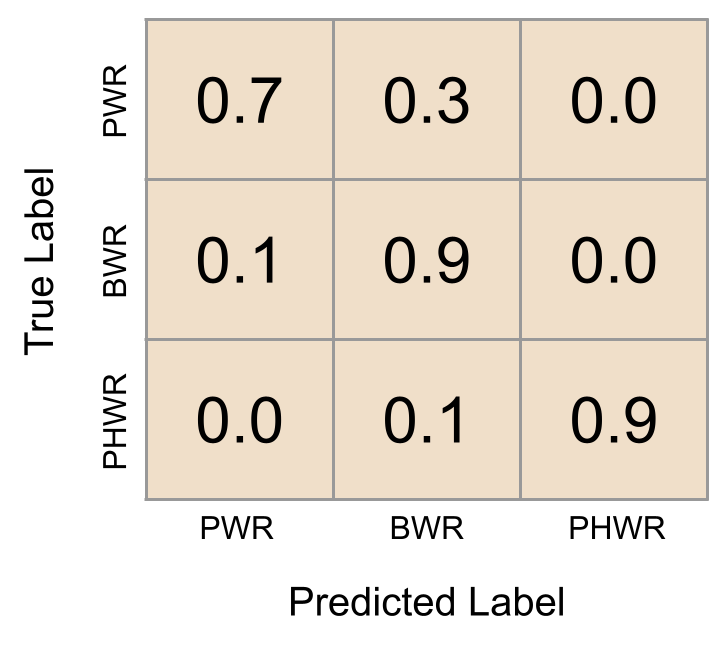
\includegraphics[width=0.35\linewidth]{./figures/cm_example.png}
  \end{figure}}
\end{frame}

\begin{frame}
  \frametitle{Performance Measures for Regression}
  \textbf{Regression Metrics:} \cite{scikit}
  \vspace{2mm}
  \begin{itemize}\addtolength{\itemsep}{0.4\baselineskip}
    \item \uncover<1->{Mean Absolute Error:\\ \vspace{2mm}
          $\textit{MAE} = \frac{1}{N_{\text{samples}}} \sum_{i=1}^{N_{\text{samples}}} \left| y_{true, i} - y_{pred, i} \right|$}
    \item \uncover<2->{Median Absolute Error:\\ \vspace{2mm}
          $\textit{MedAE} = \text{median}(\mid y_{true, 1} - y_{pred, 1} \mid, \ldots, 
                                          \mid y_{true, n} - y_{pred, n} \mid)$}
    \item \uncover<3->{Mean Absolute Percentage Error:\\ \vspace{2mm}
          $\textit{MAPE} =  \frac{100}{N_{\text{samples}}} \cdot 
                            \sum_{i=1}^{N_{\text{samples}}}
                            \frac{\left| y_{true, i} - y_{pred, i} \right|}{y_{true, i}}$}
  \end{itemize}
\end{frame}

\begin{frame}
  \frametitle{Methodology Summary}
  \begin{adjustwidth}{-10pt}{-10pt}
  \begin{minipage}{0.51\textwidth}
    \begin{figure}
      \centering
      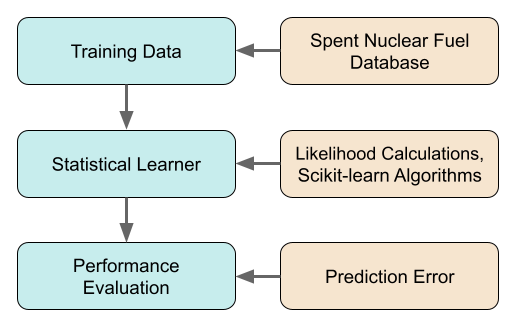
\includegraphics[width=\textwidth]{./figures/meth_pres.png}
    \end{figure}
  \end{minipage}%
  %\hfill
  \begin{minipage}{0.51\textwidth}
    \begin{itemize}
      \item Training Data: SNF recipes from SCALE/ORIGEN-ARP \cite{scale, origen}
      \item Statistical Methods
        \begin{itemize}
          \item Scikit-learn algorithms (kNN \& Decision Trees) \cite{scikit}
          \item Maximum log-likelihood calculation method \cite{mll_method, mll_sensitivity}
        \end{itemize}
      \item Performance
        \begin{itemize}
          \item Prediction error analysis
          \item \textit{Covered later: Test cases from SFCOMPO} \cite{sfcompo}
        \end{itemize}
    \end{itemize}
  \end{minipage}
  \end{adjustwidth}
\end{frame}

